\chapter{successioni ricorsive}
\label{ch:successioni_ricorsive}

Nella maggior parte di questo capitolo prenderemo in considerazione le successioni $a_n$
definite \emph{per ricorrenza} o \emph{ricorsivamente} dalle condizioni:
\index{successioni!ricorsive}
\index{successioni!definite per ricorrenza}
\index{ricorsione}
\begin{equation}\label{eq1}
\begin{cases}
  a_0 = \alpha,\\
  a_{n+1} = f(a_n)
\end{cases}
\end{equation}

Fissato il termine iniziale $\alpha$ e la legge di ricorrenza $f$,
c'è una unica successione che soddisfa \eqref{eq1} e i suoi termini
sono:
\begin{align*}
a_0 & =\alpha,\\
a_1 &= f(a_1)=f(\alpha),\\
a_2 &= f(a_2)=f(f(\alpha)),\\
a_3 &= f(a_3)=f(f(f(\alpha))),\\
&\ \vdots\\
a_n &= f(a_{n-1}) = f^n(\alpha),\\
&\ \vdots
\end{align*}


Il valore di $a_n$ potrebbe rappresentare lo stato di un sistema che
si evolve a partire da uno stato iniziale $a_0=\alpha$ tramite la
funzione $f$ che rappresenta il cambiamento di stato.
Il numero naturale $n$ potrebbe quindi rappresentare un passo temporale.
In tal senso \eqref{eq1} si chiama anche \myemph{sistema!dinamico!discreto}.

L'equazione $a_{n+1} = f(a_n)$ viene chiamata una \emph{equazione ricorsiva autonoma del primo ordine}.
Ci sono altre tipologie di equazioni che considereremo
solo marginalmente nei capitoli successivi.
Ad esempio quando abbiamo definito
il fattoriale: $a_n = n!$ abbiamo dato le condizioni:
\[
\begin{cases}
  a_0 = 1\\
  a_{n+1} = (n+1) \cdot a_n
\end{cases}
\]
ma l'equazione $a_{n+1} = (n+1) \cdot a_n$ è della forma $a_{n+1} =
f(n, a_n)$ e si dice essere \emph{non autonoma} perché la funzione di
ricorrenza $f$ dipende esplicitamente da $n$ oltre che dal termine
precedente $a_n$.

Si potrebbero anche considerare equazioni di ordine maggiore del
primo. Ad esempio la successione $F_n$ di \emph{Fibonacci}
(Leonardo Pisano, 1170--1242)
i cui primi termini sono riportati nella tabella~\ref{tab:Fibonacci}
\begin{table}
  \begin{center}
  0, 1, 1, 2, 3, 5, 8, 13, 21, 34, 55, 89, 144,
  233, 377, 610, 987\dots
\end{center}
\caption{I primi termini della succession di Fibonacci.
Ogni termine è la somma dei due precedenti.}
\label{tab:Fibonacci}
\end{table}
\mymargin{Fibonacci}%
\index{Fibonacci!successione di}%
\index{successione!di Fibonacci}%
soddisfa l'equazione ricorsiva:
\begin{equation}\label{eq:Fibonacci}
\begin{cases}
  F_0 = 0 \\
  F_1 = 1 \\
  F_{n+2} = F_{n+1} + F_n
\end{cases}
\end{equation}
che è una relazione del secondo ordine in quanto ogni termine può
essere definito utilizzando i valori dei \emph{due} termini precedenti.
Se l'equazione è lineare, come in questo caso, si possono trovare delle
formule esplicite per scrivere l'$n$-esimo termine della successione.
Lo faremo nella sezione~\ref{sec:ricorrenza_lineare}

Si potrebbero anche considerare i sistemi di equazioni ricorsive.
Ad esempio se $f$ fosse una funzione complessa $f\colon \CC \to \CC$,
$f(x+iy) = f_1(x,y) + i f_2(x,y)$ con $f_1,f_2 \colon \RR\to\RR$
si potrebbe scrivere $a_n = x_n + i y_n$ con $x_n, y_n \in \RR$
l'equazione ricorsiva $a_{n+1} = f(a_n)$
diventerebbe un sistema di due equazioni:
\[
  \begin{cases}
    x_{n+1} = f_1(x_n, y_n)\\
    y_{n+1} = f_2(x_n, y_n).
  \end{cases}
\]
Lo studio dei sistemi va oltre gli scopi di questo capitolo,
ma accenneremo solamente ad un esempio nella sezione~\ref{sec:mandelbrot}.

\section{equazioni ricorsive autonome del primo ordine}

\begin{example}[algoritmo di Erone]\label{ex_Erone}
\index{Erone!algoritmo di}%
\index{algoritmo!di Erone}%
\index{algoritmo!calcolo della radice $n$-esima}%
\index{radice $n$-esima!algoritmo di Erone}%
  Fissato un numero reale $p>1$ consideriamo la successione definita
  per
ricorrenza da
\[
\begin{cases}
  a_0 = p\\
  a_{n+1} = \frac{a_n + p/a_n}{2}.
\end{cases}
\]
Si dimostri che $a_n \to \sqrt p$.
\end{example}
Osserviamo, ad esempio, che per $p=2$ i
primi termini della successione sono:
\begin{align*}
a_0 &= 2, \\
a_1 &= \frac{2+2/2}{2} = 3/2 = 1.5, \\
a_2 &= \frac{3/2 + 2/(3/2)}{2} = 17/12 \approx 1.4166666, \\
a_3 &= \frac{17/12 + 2/(17/12)}{2} = 577 / 408 \approx 1.4142157,\\
\vdots
\end{align*}
che effettivamente \emph{sembrano} avvicinarsi molto al numero
\[
\sqrt 2\approx 1.4142135.
\]

\begin{proof}
\emph{Passo 1.} Dimostriamo per induzione che $a_n>0$ per ogni $n\in \NN$.
Infatti per $n=1$ osserviamo che $a_0=p>0$ mentre se supponiamo che
$a_n>0$ otteniamo che $a_{n+1} = \frac{a_n + \frac p {a_n}}2$ è positivo in quanto
è la metà della somma di due quantità positive. Quindi, applicando il
principio di induzione, possiamo concludere che $a_n>0$ per ogni $n$.

Abbiamo in effetti identificato un insieme $A=\ENCLOSE{x\colon x>0} = (0,
+\infty)$ tale che la funzione $f(x) = \frac{x + \frac p x}{2}$ è definita
su $A$ e, contemporaneamente, ha valori in $A$.
Quindi questo passaggio è fondamentale anche solo per
garantire che la successione $a_n$ sia ben definita.

\emph{Passo 2.} Dimostriamo che la successione $a_n$ è decrescente.
Per fare questo osserviamo che essere decrescente significa:
$ a_{n+1} \le a_n$
e cioé
\[
\frac{a_n + \frac p {a_n}}{2} \le a_n
\]
ovvero (moltiplicando ambo i lati per $a_n>0$)
\[
a_n^2 + p \le 2 a_n^2
\]
che è equivalente a $a_n^2 - p \ge 0$. E, in effetti, questa
disuguaglianza è sempre vera in quanto per $n=1$ si riduce a $a_1^2 - p
= p^2 - p \ge 0$ che è soddisfatta nel caso $p>1$. Mentre
\begin{align*}
a_{n+1}^2 - p & = \left(\frac{a_n+\frac p{a_n}}{2}\right)^2 - p
= \frac{a_n^4 + 2 p a_n^2 + p^2 - 4 p a_n^2}{4 a_n^2} \\
& = \frac{a_n^2 - 2 p a_n^2 + p^2}{4 a_n^2}
 = \frac{\left(a_n^2 - p\right)^2}{4a_n^2} \ge 0.
\end{align*}
Dunque $a_{n+1}^2 \ge p$ per ogni $n\in \NN$ e di conseguenza $a_n$ è
decrescente e inoltre $a_n > \sqrt p$.

\emph{Passo 3.}
Visto che $a_n$ è una successione decrescente,
per il teorema sulle successioni monotòne possiamo
affermare che $a_n$ ammette limite, e cioé: $a_n \to \ell$ con $\ell
\in [-\infty, +\infty]$. Possiamo immediatamente escludere
$\ell=+\infty$ in quanto la successione è decrescente, e possiamo
anche escludere $\ell<\sqrt{p}$ in quanto sappiamo che $a_n > \sqrt{p}$ e quindi
(per il teorema della permanenza del segno) $\ell \ge \sqrt p$.
Inoltre
\[
  a_{n+1} = \frac{a_n + \frac p{a_n}}{2} \to \frac{\ell + \frac p \ell}{2}.
\]
Ma sappiamo che se $a_n\to \ell$ anche $a_{n+1}\to \ell$ (visto che
$a_{n+1}$ è una sottosuccessione di $a_n$) e quindi (per l'unicità del
limite)
\begin{equation}\label{ex_1_fixed}
  \ell = \frac{\ell + \frac p \ell}{2}
\end{equation}
da cui si ricava $\ell^2 = p$ ovvero (essendo $\ell\ge 0$) concludiamo
$a_n \to \ell =
\sqrt p$.
\end{proof}

Cominciamo ora a definire una terminologia e a fissare alcuni
risultati generali che ci serviranno per trovare alcune proprietà
delle successioni definite da~ \eqref{eq1}.

\begin{definition}[punto fisso]
\mymark{**}
  Diremo che $x$ è un \myemph{punto!fisso}
  per la funzione $f$ se vale
  \[
    f(x) = x.
  \]
\end{definition}
Osserviamo che se $\alpha$ è un punto fisso per $f$ la successione costante
$a_n=\alpha$ soddisfa l'equazione $a_{n+1} = f(a_n)$. Inoltre se
$a_{n+1} = f(a_n)$, se $a_n$ converge ad un limite $\ell$ e se
$f$ è continua in $\ell$ allora
\[
a_{n+1} = f(a_n) \to f(\ell)
\]
ma visto che $a_{n+1}$ ha lo stesso limite di $a_n$ si trova che
$f(\ell)=\ell$ ovvero il limite della successione è un punto fisso.

Nell'esempio precedente la funzione $f(x) = \frac{x+\frac p x}2$ ha come punti
fissi $\sqrt{p}$ e $-\sqrt{p}$ e l'equazione~\eqref{ex_1_fixed} non è
altro che $f(x)=x$. E in effetti abbiamo mostrato che la successione
$a_n$ converge proprio ad un punto fisso.

\begin{definition}[insieme invariante]
\mymark{**}
  Un insieme $A$ si dice essere \emph{invariante}
  \mynote{insieme invariante}
  per $f$ se
  $f(A)\subseteq A$
  (ovvero: per ogni $x\in A$ si ha $f(x)\in A$).
\end{definition}

Osserviamo che se $A$ è un insieme invariante e $a_0\in A$ allora la
successione definita da $a_{n+1}=f(a_n)$ assume sempre valori in $A$.

Nell'esercizio~\ref{ex_Erone} abbiamo dimostrato che gli intervalli
$(0,+\infty)$ e $(\sqrt{p},+\infty)$ sono invarianti.

\begin{theorem}\label{th_1}
\mymark{*}
  Sia $A\subset \RR$ un insieme invariante per $f$ e sia $a_n$ una
  successione con $a_1 \in A$ e $a_{n+1}=f(a_n)$.

  Se per ogni $x\in A$
  vale $f(x) \ge x$
  \mynote{$f(x)\ge x$}
  allora la successione $a_n$ è crescente.

  Se per ogni $x\in A$ vale $f(x) \le x$
  \mynote{$f(x)\le x$}
  allora la successione $a_n$ è decrescente.
\end{theorem}
\begin{proof}
\mymark{*}
  In effetti se $f(x) \ge x$ si ha per ogni $n\in \NN$
  \[
  a_{n+1} = f(a_n) \ge a_n
  \]
e quindi la successione $a_n$ è crescente. Mentre se $f(x) \le x$ si ha
  \[
  a_{n+1} = f(a_n) \le a_n
  \]
e la successione è decrescente.
\end{proof}

\begin{exercise}
Al variare di $\alpha \in \RR$
determinare il limite della successione $a_n$ definita per ricorrenza dalle
equazioni:
\[
\begin{cases}
 a_1 = \alpha \\
 a_{n+1} = a_n - a_n^2.
\end{cases}
\]
\end{exercise}

\begin{theorem}
\mymark{**}
  Sia $A\subset \RR$ un insieme invariante per $f$ e sia $a_n$ una successione
  con $a_0\in A$ e $a_{n+1} = f(a_n)$. Se $f$ è crescente
  \mynote{$f$ crescente}
  su $A$ allora $a_n$
  è monotòna.
\end{theorem}
\begin{proof}
\mymark{**}
  Osserviamo che se $f$ è crescente allora
  \begin{align*}
    a_{n+1} \ge a_n \Rightarrow f(a_{n+1}) \ge f(a_n) \Rightarrow
    a_{n+2} \ge a_{n+1}\\
    a_{n+1} \le a_n \Rightarrow f(a_{n+1}) \le f(a_n) \Rightarrow a_{n+2} \le a_{n+1}.
  \end{align*}
  Dunque se per i primi due termini si ha $a_1 \ge a_0$ allora, per
  induzione, si ha $a_{n+1} \ge a_n$ per ogni $n$ e quindi la
  successione è crescente. Se invece $a_2 \le a_1$ si dimostra per
  induzione che $a_{n+1} \le a_n$ per ogni $n$ e quindi la successione
  è decrescente.
\end{proof}

\begin{theorem}\label{th_decr}
\mymark{**}
  Sia $A\subset \RR$ un insieme invariante per $f$ e sia $a_n$ una successione
  con $a_1\in A$ e $a_{n+1} = f(a_n)$. Se $f$ è decrescente
  \mynote{$f$ decrescente}
  su $A$
  allora le due successioni $a_{2n}$ (termini di indice pari) e
  $a_{2n+1}$ (termini di indice dispari) sono monotòne.
\end{theorem}
\begin{proof}
\mymark{**}
  Osserviamo che
  \begin{align*}
    a_{2n+2} &= f(a_{2n+1}) = f(f(a_{2n})) = (f\circ f)(a_{2n})\\
    a_{2n+3} &= f(a_{2n+2}) = f(f(a_{2n+1})) = (f\circ f)(a_{2n+1})
  \end{align*}
cioé le sottosuccessioni dei termini di indice pari e di indice
dispari soddisfano una relazione di ricorrenza tramite la funzione
$f\circ f$ (invece che $f$).

Osserviamo anche che se $f$ è decrescente allora $f\circ f$ è
crescente. Infatti:
\[
x \le y \Rightarrow f(x) \ge f(y) \Rightarrow f(f(x)) \le f(f(y)).
\]

Dunque possiamo applicare il teorema precedente e ottenere che le due
sottosuccessioni sono entrambe monotòne.
\end{proof}

Utilizziamo la terminologia e i risultati precedenti nei seguenti
esercizi.

\begin{exercise}[Fibonacci]\label{ex_fibonacci}
\index{Fibonacci!successione di}
\index{successione!di Fibonacci}
  Si consideri il rapporto $a_n = \frac{F_{n+1}}{F_n}$ di due termini
  successivi della successione di Fibonacci: $F_0=1$, $F_1=1$,
  $F_{n+2} = F_{n+1} + F_n$. Determinare il limite di $a_n$.
\end{exercise}

\begin{proof}[Soluzione]
  La successione $a_n$ soddisfa la relazione:
  \[
   a_{n+1} = \frac{F_{n+2}}{F_{n+1}} = \frac{F_{n+1}+F_n}{F_{n+1}} = 1
   + \frac{F_n}{F_{n+1}} = 1 + \frac{1}{a_n}.
   \]
   Inoltre $a_0=F_2 / F_1 = 1$. Dunque la successione $a_n$ soddisfa
   le seguenti proprietà:
   \[
   \begin{cases}
     a_0 = 1 \\
     a_{n+1} = 1 + \frac{1}{a_n}.
   \end{cases}
   \]

   Osserviamo che l'intervallo $A=(0,+\infty)$ è invariante per la
   funzione $f(x) = 1+1/x$. Infatti
   se $x\in A$ allora $x>0$ ma anche $f(x) = 1+1/x$ lo è.
   Su tale intervallo, inoltre, la funzione $f$ è decrescente. Infatti
   \[
   0 < x \le y \Rightarrow \frac 1 x \ge \frac 1 y \Rightarrow 1+\frac
   1 x \ge 1 + \frac 1 y
   \Rightarrow f(x) \ge f(y).
   \]
   Visto che $a_0 = 1 \in A$, $A$ invariante, $f$ decrescente su $A$,
   il Teorema~\ref{th_decr} ci dice che le due successioni $a_{2n}$ e
   $a_{2n+1}$ sono monotone e quindi ammettono limite: $a_{2n}\to
   \ell$, $a_{2n+1} \to \ell'$ con $\ell,\ell' \in [0,+\infty]$.

   Se $\ell$ è finito si ha:
   \[
   a_{2n+1} = f(a_{2n}) = 1+ \frac{1}{a_{2n}} \to 1 + \frac{1}{\ell}
   \]
   e quindi dato che $a_{2n+1}\to \ell'$ si ha $\ell' = 1 + 1/\ell$.
   Inoltre
   \begin{align*}
   a_{2n+2} &= f(a_{2n+1}) = 1 + \frac{1}{a_{2n+1}} \to 1 +
   \frac{1}{\ell'}
   = 1 + \frac{1}{1+\frac{1}{\ell}} \\
   & = 1 + \frac{\ell}{\ell+1}
   = \frac{2\ell +1}{\ell +1}
   \end{align*}
   da cui, visto che $a_{2n+2}\to \ell$,
   \[
   \ell = \frac{2\ell +1 }{\ell +1}.
   \]
   Moltiplicando ambo i membri per $\ell+1$ si ottiene
   \[
    \ell^2 + \ell = 2\ell + 1
    \]
    ovvero $\ell^2 - \ell -1 =0$ da cui, utilizzando la formula
    risolutiva delle equazioni di secondo grado, e ricordando che
    $\ell \ge 0$, si trova:
    \[
    \ell = \frac{1 + \sqrt{5}}{2}.
    \]
    Ma anche
    \begin{align*}
    \ell' &= 1 + \frac 1 \ell = \frac{\ell + 1}{\ell} = \frac{3+\sqrt
      5}{1 + \sqrt 5} = \frac{(3+\sqrt 5)(1-\sqrt 5)}{1-5} \\
     &= \frac{3-2\sqrt 5-5}{-4} = \frac{2+2\sqrt 5}{4} = \frac{1+\sqrt
       5}{2} = \ell.
    \end{align*}
    Dunque entrambe le sottosuccessioni dei termini di indice pari e
    di indice dispari convergono allo stesso valore $\ell$ e quindi
    l'intera successione ci converge: $a_n\to (1+\sqrt 5)/2$.

    Il caso $\ell=+\infty$ si può escludere in quanto ripetendo il
    ragionamento fatto sopra si otterrebbe $\ell' = 1$ da cui:
    $\ell = 1 + 1/\ell' = 2$ che è una contraddizione.
\end{proof}

\begin{figure}
  \myurl{fibonacci}{Diagramma a ragnatela relativo all'esercizio \getrefnumber{ex_fibonacci}}
  \begin{center}
    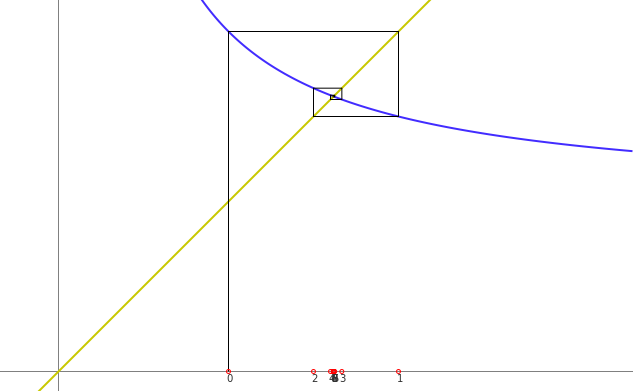
\includegraphics[width=\textwidth]{fig_fibonacci.png}
  \end{center}
  \caption{Diagramma a ragnatela relativo
    all'esercizio~\ref{ex_fibonacci}:
    sul rapporto dei termini successivi della successione di Fibonacci.}
  \label{fig_fibonacci}
\end{figure}

Un metodo grafico per visualizzare l'andamento dei termini della
successione definita da \eqref{eq1} è il \emph{diagramma a
  ragnatela}. Si disegna la curva $y=f(x)$ su un piano
cartesiano. Partendo dal punto di coordinate $(\alpha, 0)=(a_0, 0)$ si procede
lungo una retta verticale fino a raggiungere il grafico della funzione
nel punto $(a_0, f(a_0)) = (a_0, a_1)$.
Dopodiché si procede in
orizzontale fino ad incontrare la retta $y=x$ nel punto $(a_1,a_1)$ e
si ripete il procedimento in modo che le coordinate $x$ (ma anche le $y$)
dei vertici della spezzata mi danno la successione $a_0, a_1, a_2,
\dots$. Ad esempio il diagramma a ragnatela corrispondente
all'esercizio~\ref{ex_fibonacci} è rappresentato in
Figura~\ref{fig_fibonacci}.

\begin{exercise}\label{ex_3}
  Si consideri la successione definita per ricorrenza
  \[
  \begin{cases}
    a_0 = 0\\
    a_{n+1} =1 + a_n^2.
  \end{cases}
  \]
  Determinare il limite della successione.
\end{exercise}

\begin{figure}
  \myurl{ex3}{Diagramma a ragnatela relativo all'esercizio \getrefnumber{ex_3}}
  \begin{center}
    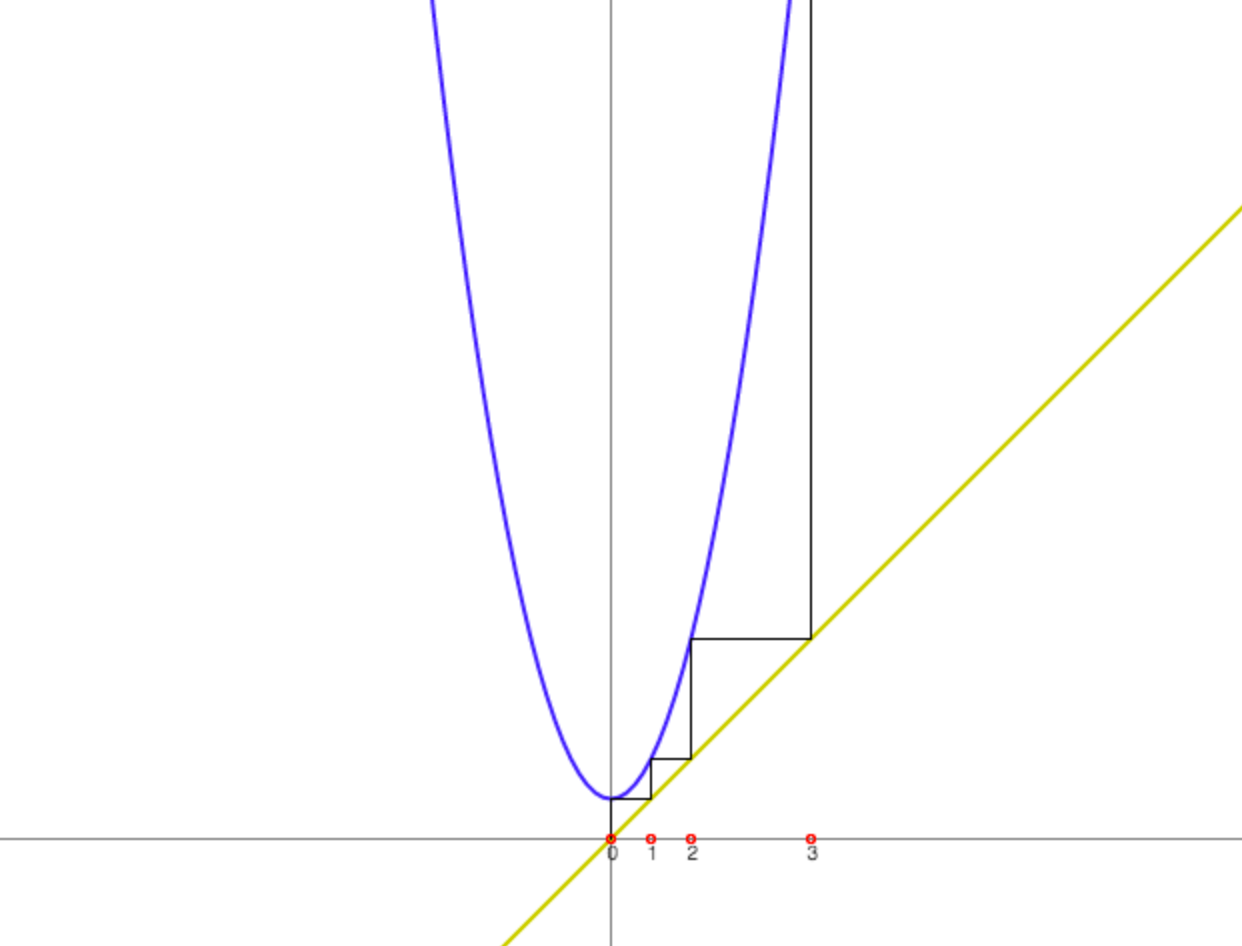
\includegraphics[width=\textwidth]{fig_ex_3.png}
  \end{center}
  \caption{Diagramma a ragnatela relativo
    all'esercizio~\ref{ex_3}.}
  \label{fig_ex_3}
\end{figure}

\begin{proof}[Soluzione]
  L'equazione ricorsiva è $a_{n+1}=f(a_n)$ se poniamo $f(x) = 1+x^2$.
  E' facile verificare che per ogni $x$ si ha $f(x) > x$ e quindi, per
  il Teorema~\ref{th_1} otteniamo che la successione $a_n$ è
  crescente. Dunque ammette limite: $a_n \to \ell$. Se il limite fosse
  finito si avrebbe
  \[
  a_{n+1} = 1 + a_n^2 \to 1 + \ell^2
  \]
  e quindi, visto che $a_{n+1}\to \ell$, si avrebbe $\ell = 1 +
  \ell^2$ (cioè $\ell$ dovrebbe essere un punto fisso di $f$). Questa
  equazione abbiamo già osservato che non ha soluzioni ($x^2 + 1 > x$)
  e quindi $\ell$ non è finito. Visto che la successione $a_n$ è
  crescente possiamo escludere che sia $\ell=-\infty$ e quindi l'unica
  possibilità che rimane è che $a_n \to +\infty$.
\end{proof}

\begin{figure}
  \myurl{ex4}{Diagramma a ragnatela relativo all'esercizio \getrefnumber{ex_4}}
  \begin{center}
  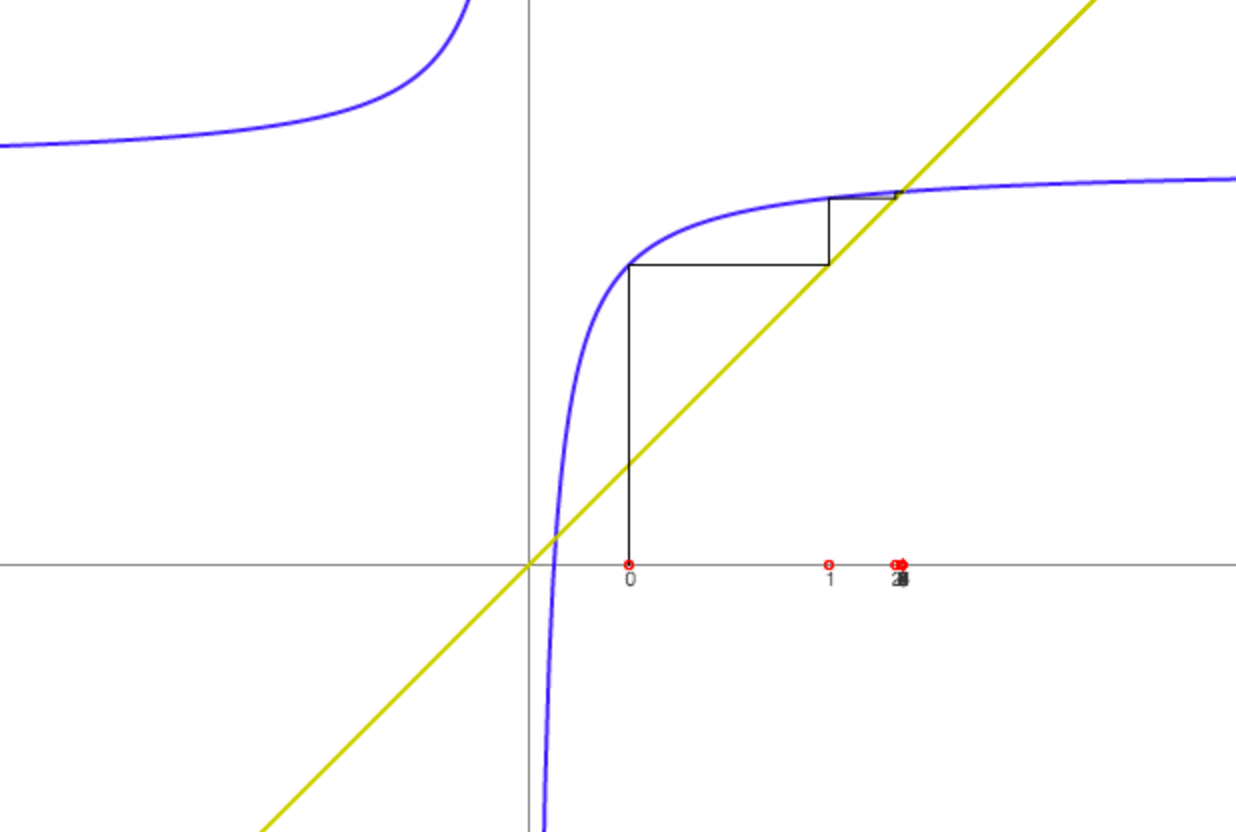
\includegraphics[width=\textwidth]{fig_ex_4.png}
  \end{center}
  \caption{Diagramma a ragnatela relativo
    all'esercizio~\ref{ex_4}.}
  \label{fig_ex_4}
\end{figure}

\begin{exercise}\label{ex_4}
  Si consideri la successione definita per ricorrenza
  \[
  \begin{cases}
    a_0 = 1\\
    a_{n+1} =4-\frac 1 {a_n}.
  \end{cases}
  \]
  Determinare il limite della successione.
\end{exercise}

\begin{proof}[Soluzione.]
  Si mostra che sull'intervallo $A=(2-\sqrt 3, 2+\sqrt 3)$
  vale $f(x)>x$, che gli estremi di $A$ sono punti fissi
  e inoltre che la funzione $f$ è crescente (lo è su tutto $(0,+\infty)$).
  Di conseguenza è facile verificare che $A$ è invariante, in quanto si ha
  \begin{align*}
  2-\sqrt 3 < x < 2+\sqrt 3 &\Rightarrow
  f(2-\sqrt 3) < f(x) < f(2+\sqrt 3)\\
  &\Rightarrow
  2-\sqrt 3 < f(x) < 2+\sqrt 3.
  \end{align*}

  Inoltre se $a_0 \in A$ allora per ogni $n\in\NN$ si ha $a_n\in A$ ed essendo
  $f(x)>x$ la successione sarà crescente. Dunque ammette
  limite: $a_n \to \ell \in [2-\sqrt 3,2+\sqrt 3]$, $\ell \ge a_0$.
  Ma allora
  \[
  a_{n+1} = 4-\frac 1 {a_n} \to 4 - \frac 1 \ell = f(\ell)
  \]
  e visto che $a_{n+1}$ ha lo stesso limite di $a_n$ si ha $\ell =
  f(\ell)$ le cui uniche soluzioni sono $2\pm \sqrt 3$. Ma $2-\sqrt 3$
  va scartata in quanto $\ell\ge a_0 > 2-\sqrt 3$ e quindi rimane
  $a_n \to \ell = 2+\sqrt 3$.
\end{proof}

\begin{figure}
 \myurl{ex5}{Diagramma a ragnatela relativo all'esercizio \getrefnumber{ex_5}}
 \begin{center}
    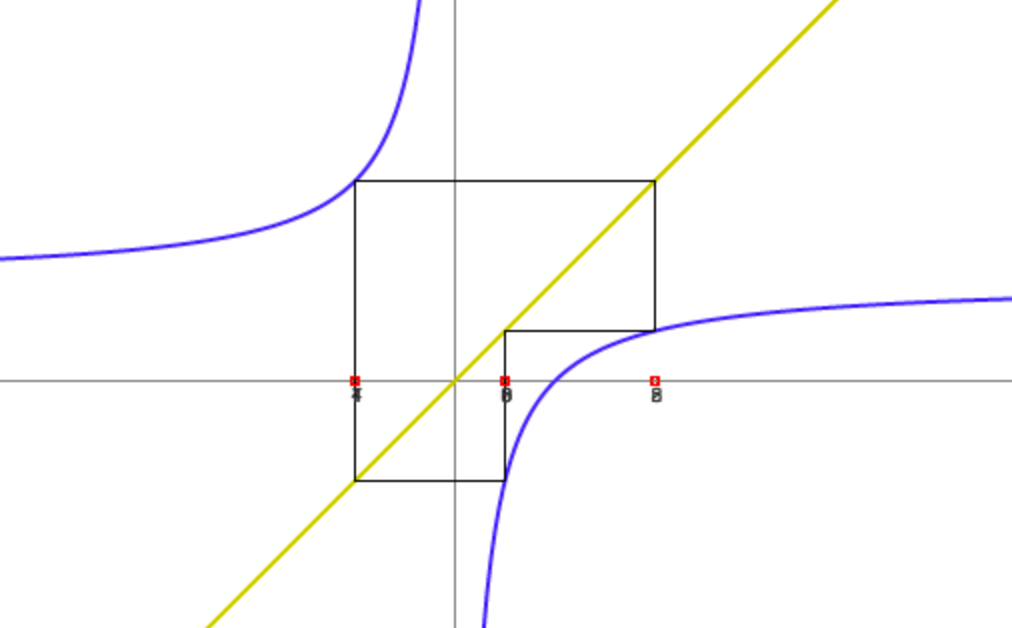
\includegraphics[width=\textwidth]{fig_ex_5.png}
  \end{center}
  \caption{Diagramma a ragnatela relativo
    all'esercizio~\ref{ex_5}.}
  \label{fig_ex_5}
\end{figure}

\begin{exercise}\label{ex_5}
  Si consideri la successione definita per ricorrenza
  \[
  \begin{cases}
    a_0 = \frac 1 2\\
    a_{n+1} = 1- \frac{1}{a_n}
  \end{cases}
  \]
  Determinare, se esiste, il limite della successione.
\end{exercise}

\begin{proof}[Soluzione.]
  Osserviamo che:
  \begin{align*}
    a_0 &= \frac 1 2 \\
    a_1 &= 1 - \frac{1}{1/2} = -1\\
    a_2 &= 1 - \frac{1}{-1} = 2\\
    a_3 &= 1 - \frac{1}{2} = \frac 1 2 = a_0
  \end{align*}
  Essendo $a_3 = a_0$ la successione si ripete e, (per induzione) si
  dimostra che $a_{3n+k} = a_k$. Dunque si ha
  \begin{align*}
    a_{3n} &= a_0 = \frac 1 2\\
    a_{3n+1} &= a_1 = -1\\
    a_{3n+2} &= a_2 = 2
  \end{align*}
  e la successione $a_n$ non ammette limite.
\end{proof}

\begin{figure}
  \myurl{ex6}{Diagramma a ragnatela relativo all'esercizio \getrefnumber{ex_6}}
  \begin{center}
    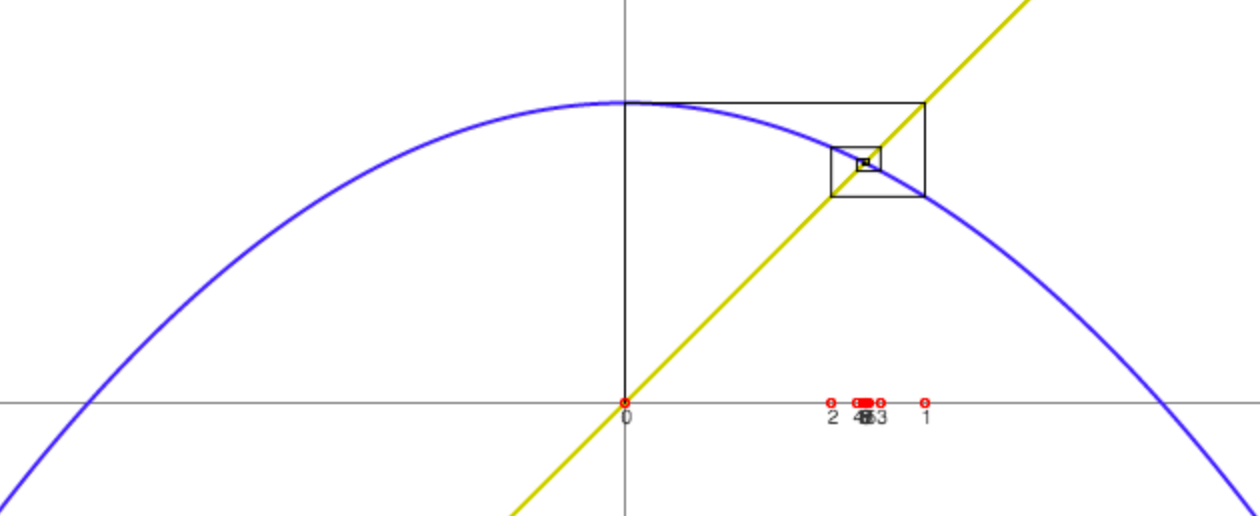
\includegraphics[width=\textwidth]{fig_ex_6.png}
  \end{center}
  \caption{Diagramma a ragnatela relativo
    all'esercizio~\ref{ex_6}.}
  \label{fig_ex_6}
\end{figure}

\begin{exercise}\label{ex_6}
  Si consideri la successione definita per ricorrenza
  \[
  \begin{cases}
    a_0 = 0\\
    a_{n+1} = \frac{5-a_n^2}{4}.
  \end{cases}
  \]
  Determinare il limite della successione.
\end{exercise}

\begin{proof}[Soluzione.]
Si ha $a_{n+1} = f(a_n)$ se scegliamo $f(x) = (5-x^2)/4$. Osserviamo
che la funzione $f$ è decrescente per $x \ge 0$ (infatti $0 \le x_1 <
x_2$ implica $x_1^2 < x_2^2$ da cui $-x_1^2 > -x_2^2$ e quindi $f(x_1)
> f(x_2)$). Osserviamo inoltre che
\begin{align*}
a_0 &= 0\\
a_1 &= f(a_1) = \frac 5 4.\\
a_2 &= f\enclose{\frac 5 4} = \frac{5-25/16}{4} = \frac{55}{64}
\end{align*}
Vogliamo dimostrare che l'intervallo $A=[0,5/4]$ è invariante. Visto
che $f$ è decrescente su tale intervallo, si ha:
\begin{align*}
0 \le x \le \frac 5 4 &\Rightarrow f(0) \ge f(x) \ge f(5/4)\\
&\Rightarrow \frac 5 4 \ge f(x) \ge \frac{55}{64} \ge 0\\
&\Rightarrow 0 \le f(x) \le \frac 5 4
\end{align*}
cioè $x\in A \Rightarrow f(x)\in A$, che è quanto volevamo dimostrare.

Per il Teorema~\ref{th_decr} sappiamo dunque che $a_{2n} \to \ell$ e
$a_{2n+1} \to \ell'$. Entrambi i limiti sono finiti in quanto essendo
$a_n \in A$ per ogni $n$, si ha $\ell, \ell' \in \bar A = A$.
Dunque, come al solito, osserviamo che si ha:
\begin{align*}
  a_{2n+1} &= f(a_n) \to f(\ell)  \\
  a_{2n+2} &= f(a_{n+1}) \to f(\ell')
\end{align*}
ma sapendo che $a_{2n+1}\to \ell'$ e $a_{2n+2}\to \ell$ otteniamo il
seguente sistema:
\[
\begin{cases}
  \ell' = f(\ell)\\
  \ell = f(\ell')
\end{cases}
\]
da cui si ottiene $f(f(\ell))=\ell$ e $f(f(\ell'))=\ell'$. Dunque
vogliamo scrivere e risolvere l'equazione $f(f(x))=x$:
\[
\frac{5-\left(\frac{5-x^2}{4}\right)^2}{4} = x
\]
cioè
\[
5 - \frac{25 - 10x^2 + x^4}{16} = 4x
\]
ovvero
\[
x^4 - 10 x^2 + 64 x - 55 = 0.
\]

Come facciamo a risolvere una equazione di quarto grado?
In questo frangente dobbiamo fare una osservazione di carattere
generale che ci sarà di grande aiuto.
Osserviamo che se $x$ è una soluzione di $f(x)=x$ allora $x$
è anche soluzione di $f(f(x)) = x$ in quanto in tal caso si ha
$f(f(x))=f(x)=x$.
Ma l'equazione $f(x) = x$ è una equazione di secondo grado, che quindi
possiamo facilmente risolvere:
\begin{gather*}
  \frac{5-x^2}{4} = x \\
  x^2 + 4x - 5 = 0 \\
  x_{12} = -2 \pm \sqrt{4 + 5} = -2 \pm 3.
\end{gather*}

Dunque abbiamo trovato due zeri del polinomio di quarto grado e
tale polinomio deve essere quindi divisibile per
\[
 x^2 + 4x - 5 = (x-1)(x+5).
\]
Eseguiamo la divisione tra polinomi:
\begin{align*}
\frac{x^4 - 10 x^2 + 64 x - 55}{x^2 + 4x - 5}
&= x^2 + \frac{x^4 - 10 x^2 + 64x - 55 - x^2 (x^2 + 4x - 5)}{x^2+4x-5}\\
&= x^2 + \frac{-4x^3 - 5 x^2 + 64 x - 55}{x^2+4x-5}\\
&= x^2 - 4x + \frac{-4x^3 - 5x^2 - 64 x - 55 + 4x(x^2+4x-5)}{x^2+4x-5}
\\
&= x^2 - 4x + \frac{11 x^2 + 44 x - 55}{x^2 + 4x -5}\\
&= x^2 - 4x + 11.
\end{align*}
Come previsto la divisione non ha resto. Possiamo quindi completare la
scomposizione cercando gli zeri del polinomio $x^2-4x+11$ che però, da
un rapido controllo, non ha soluzioni reali.

Dunque in questo caso i punti fissi di $f$ coincidono con i punti
fissi di $f\circ f$ e dunque i due limiti $\ell, \ell'$ devono essere
elementi dell'insieme dei punti fissi: $\ENCLOSE{1, -5}$. D'altra parte $-5$
deve essere escluso in quanto i limiti stanno entrambi nella chiusura
dell'insieme invariante, che non comprende numeri negativi.

Concludiamo quindi che $\ell = \ell' = 1$ e dunque l'intera
successione ha limite: $a_n \to 1$.
\end{proof}

\begin{exercise}\label{ex_7}
  Si consideri la successione definita per ricorrenza
  \[
  \begin{cases}
    a_0 = \alpha\\
    a_{n+1} = 2- a_n^2.
  \end{cases}
  \]
  Determinare il limite della successione nei casi: $\alpha=-7$, $\alpha=4$ e $\alpha=1/42$.
\end{exercise}

\begin{figure}
 \myurl{ex7}{Diagramma a ragnatela relativo all'esercizio \getrefnumber{ex_7}}
   \begin{center}
    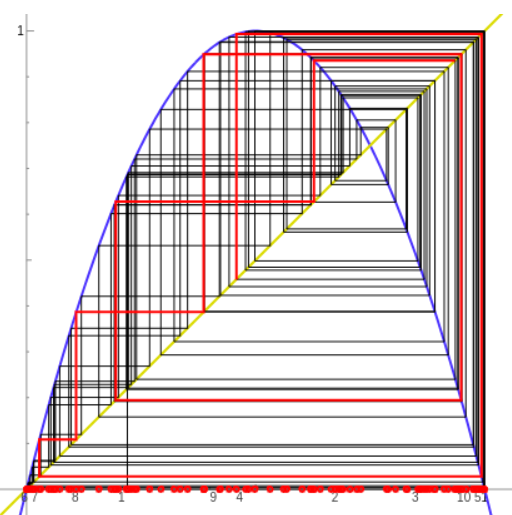
\includegraphics[width=\textwidth]{fig_ex_7.png}
  \end{center}
  \caption{Diagramma a ragnatela relativo
    all'esercizio~\ref{ex_7}.}
  \label{fig_ex_7}
\end{figure}

\begin{proof}[Soluzione.]
  Abbiamo $a_{n+1} = f(a_n)$ con $f(x) = 2-x^2$. Determiniamo i punti
  fissi di $f$:
  \[
  2-x^2 = x, \qquad x^2 + x - 2 = 0
  \]
  che ha come soluzioni $x_{1,2} = \frac{-1\pm\sqrt{1+8}}{2}$ cioé
  $x_1 = -2$, $x_2 = 1$. Tenendo conto anche dei segni si può
  osservare che all'interno delle due soluzioni si ha $f(x)>x$ mentre
  all'esterno si ha $f(x)<x$.

  Osserviamo inoltre che $f(x)$ è crescente per
  $x\le 0$ e decrescente per $x\ge 0$.

  Caso $\alpha=-7$. In questo caso consideriamo l'intervallo
  $A=(-\infty, -2)$. Visto che $f$ è crescente su questo intervallo,
  e visto che $-2$ è un punto fisso si ha:
  \[
  x < -2 \Rightarrow f(x) < f(-2) \Rightarrow f(x) < -2
  \]
  che significa che $A$ è un intervallo invariante.

  Su questo intervallo si ha $f(x)<x$ e quindi $a_n$ è decrescente e
  di conseguenza ammette limite $a_n\to \ell$. Il limite può essere
  finito oppure $-\infty$. Ma se fosse finito allora avremmo
  \[
  a_{n+1} = 2 - a_n^2 \to 2 - \ell^2
  \]
  e siccome $a_{n+1}\to \ell$ avremmo $\ell = 2 - \ell^2$ cioè $\ell$
  è un punto fisso di $f$. Ma visto che $\ell \le a_1 = \alpha < x_1 <
  x_2$ otteniamo un assurdo.

  Dunque l'unica possibilità è che $a_n \to -\infty$. Questo
  stesso ragionamento vale per ogni $\alpha<-2$.

  Caso $\alpha=4$. In questo caso si ha:
  \begin{align*}
    a_0 &= \alpha = 4\\
    a_1 &= f(a_0) = 2 - 4^2 = -14.
  \end{align*}
  quindi $a_1 \in A$ (l'intervallo invariante del punto precedente) e
  dall'indice $2$ in poi ci si riconduce quindi ai risultati
  precedenti. Dunque anche in questo caso $a_n \to -\infty$.

  Caso $\alpha = \frac 1{42}$. Questo caso è decisamente più complesso dei
  precedenti. Prendiamo l'insieme $A_2 = [-2, 2]$: vogliamo dimostrare
  che è un insieme invariante. Nell'intervallo $[-2,0]$ la funzione è
  crescente e quindi ha minimo in $-2$ dove vale $f(-2)=-2$ ed ha
  massimo in $0$ dove assume il valore $f(0) = 2$. Nell'intervallo
  $[0,2]$ la funzione è decrescente e, di nuovo, ha massimo $f(0)=2$ e
  minimo $f(2)=-2$. Dunque per ogni $x\in [-2,2]$ si ha $f(x) \in
  [-2,2]$ cioè, come volevamo dimostrare, $A_2$ è invariante.

  Dunque visto che $a_0 = \alpha \in A_2$ scopriamo che per ogni $n$
  si ha $a_n \in [-2,2]$. Supponiamo ora che la successione abbia
  limite: $a_n \to \ell$. In tal caso, passando al limite
  nell'equazione $a_{n+1} = f(a_n)$ otteniamo, come al solito, che il
  limite dovrebbe essere un punto fisso di $f$: o $\ell=-2$ oppure
  $\ell=1$. Cercheremo ora di dimostrare che questo è assurdo. Ci sono
  due possibilità che dobbiamo escludere. La prima è che la
  successione tenda al punto fisso $\ell$ senza mai uguagliarlo. La
  seconda è che per un certo $n_0$ si abbia $a_n = \ell$ per $n=n_0$ e
  quindi per ogni $n\ge n_0$.

  Supponiamo di essere nel primo caso e supponiamo che $\ell = -2$. In
  tal caso, per il teorema della permanenza del segno la successione
  deve, da un certo indice in poi, stare nell'intervallo $[-2, 0]$. Ma
  in tale intervallo si ha $f(x)>x$ e quindi la successione sarebbe,
  da un certo indice in poi, crescente. Ma visto che $a_n \ge -2$ per
  ogni $n$, non è possibile che la successione converga, crescendo, a
  $-2$.

  Supponiamo allora di essere nel primo caso (la successione è sempre
  diversa dai due punti fissi) e supponiamo che $\ell = 1$. In
  questo caso da un certo indice in poi la successione deve stare
  nell'intervallo $[0,2]$ (altrimenti non potrebbe convergere a
  $1$. In tale intervallo la funzione $f$ è decrescente e quindi
  le sottosuccessioni dei termini pari e dei termini dispari sono
  entrambe monotone. Si potrebbe cercare di studiare le successioni dei
  termini pari $a_{2n}$ e dispari $a_{2n+1}$ che soddisfano una relazione di ricorrenza
  con la funzione $f\circ f$ al posto di $f$ e osservare che la successione
  che si trova a sinistra del punto fisso dovrebbe decrescere e quella che si trova a
  destra dovrebbe crescere (e questo sarebbe assurdo). Un metodo forse più
  rapido che non richiede lo studio della funzione composta è invece il seguente.
  L'idea è di osservare che $f$ tende ad aumentare le distanze quando ci si trova
  nei paraggi del punto $1$. Se per assurdo $a_n\to 1$ allora definitivamente
  si dovrà avere $\abs{a_n-1}< 1/2$. Ma allora si osserva che:
  \[
    \abs{a_{n+1}-1}
    = \abs{2-a_n^2-1}=\abs{1-a_n^1}
    = \abs{1+a_n}\cdot \abs{1-a_n}
    \ge \frac 3 2 \abs{a_n-1}
  \]
  in quanto se $\abs{a_n-1}<1/2$ allora (per la disuguaglianza triangolare inversa)
  $\abs{1+a_n}\ge \frac 3 2$. Questo è assurdo perché significa che $\abs{a_n -1}\to +\infty$
  (per il criterio del rapporto) quando invece dovrebbe essere $\abs{a_n-1}\to 0$.

  \textbf{Nota.} Vedremo nei prossimi teoremi che
  se la derivata di $f$ è in valore assoluto minore di
  $1$ allora il punto fisso sarà stabile (o attrattivo) cioè partendo
  da un punto sufficientemente vicino si convergerà necessariamente al
  punto fisso. Se invece la derivata è in valore assoluto maggiore di
  $1$ il punto fisso sarà instabile (o repulsivo). Cioè, a parte la
  successione costante che assume il valore esatto del punto fisso,
  non è
  possibile che una successione converga al punto fisso.

  Rimane da considerare la possibilità che la successione assuma da un
  certo punto in poi il valore esatto di un punto fisso. Supponiamo ad
  esempio che per un certo $n$ si abbia $a_n=1$. Allora si deve avere
  \[
  1 = a_n = 2-(a_{n-1})^2
  \]
  da cui
  \[
  a_{n-1} = \pm 1.
  \]
  Se $a_n$ era il primo termine con valore $1$ dovrà necessariamente
  essere $a_{n-1} = -1$. Ma allora
  \[
  -1 = a_{n-1} = 2-(a_{n-2})^2
  \]
  da cui $a_{n-2} = \pm \sqrt 3$. Ma ora osserviamo che essendo $a_0=
  \alpha = \frac 1 {42}$ un numero razionale, e osservando che $\QQ$ è un
  insieme invariante per $f$ (perché? verificare per induzione...)
  sappiamo che ogni $a_k \in \QQ$ e quindi
  avremmo $a_{n_2} = \sqrt 3 \in \QQ$: assurdo.

  Stesso discorso si può fare se si avesse $a_n=-2$, in quanto si
  avrebbe $a_{n-1} = 2$, $a_{n-2} = 0$ e quindi $a_{n-3}=\pm \sqrt 2$.

  Dunque la successione $a_n$ non ammette limite.
\end{proof}

\begin{exercise}\label{ex_8}
  Si consideri la successione definita per ricorrenza
  \[
  \begin{cases}
    a_0 = \alpha\\
    a_{n+1} = \frac{1}{2-a_n}.
  \end{cases}
  \]
  Trovare il limite della successione nel caso $\alpha =
  -\the\year$. Determinare l'insieme dei valori di $\alpha$ per i quali la
  successione $a_n$ non è ben definita (in quanto per un qualche $n$ il
  denominatore $2-a_n$ si annulla).
  Trovare il limite nel caso $\alpha=\frac{\the\year}{1000}$.
\end{exercise}

\begin{figure}
 \myurl{ex8}{Diagramma a ragnatela relativo all'esercizio \getrefnumber{ex_8}}
 \begin{center}
    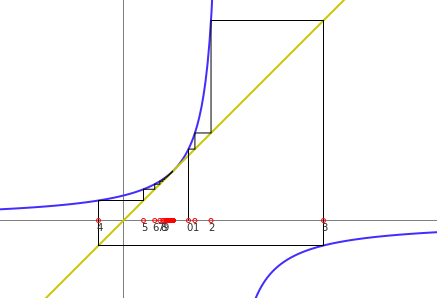
\includegraphics[width=\textwidth]{fig_ex_8.png}
  \end{center}
  \caption{Diagramma a ragnatela relativo
    all'esercizio~\ref{ex_8}.}
  \label{fig_ex_8}
\end{figure}

\begin{proof}[Soluzione.]
Posto $f(x) = 1/(2-x)$
si osserva che la disequazione $f(x)\ge x$ è verificata per ogni
$x<2$. L'equazione di punto fisso $f(x)=x$ ha come unica soluzione
$x=1$. Sull'intervallo $A=(-\infty,1)$ la funzione $f$ è crescente e
l'intervallo risulta essere invariante. Dunque per
$\alpha=-\the\year \in A$ la successione risulta essere crescente e superiormente
limitata. Dunque converge $a_n\to \ell$. Passando al limite in
$a_{n+1} = f(a_n)$ si trova che $\ell$ deve essere un punto fisso di
$f$ e quindi $\ell = 1$.

La successione non è ben definita se per qualche $n$ si trovasse
$a_n=2$ in quanto la funzione $f$ non è definita per $x=2$. Altri
valori si ottengono risalendo all'indietro la successione $a_n$.
Dalla equazione
\[
a_n = \frac{1}{2-a_{n-1}}
\]
si ricava
\[
a_{n-1} = 2-\frac{1}{a_n}.
\]
L'insieme dei punti partendo da quali si arriva prima o poi in $x=2$ è
dato dunque dai valori della successione
\[
\begin{cases}
  b_1 = 2\\
  b_{n+1} = 2 - \frac{1}{b_n}.
\end{cases}
\]
Osserviamo che in questo caso specifico è possibile ricavare una
formula esplicita per il termine $b_n$. Osserviamo infatti che:
\[
b_0 = 2,\quad
b_1 = \frac{3}{2},\quad
b_2 = \frac{4}{3}
\]
e proviamo a congetturare che sia $b_n = \frac{n+1} n$. In effetti questo
si può dimostrare per induzione. Per $n=1$ si ha $(n+1)/n = 2 =
b_1$. E se supponiamo che valga $b_n = (n+1)/n$ si ha
\[
b_{n+1} = 2 - \frac{n}{n+1} = \frac{2n+2-n}{n+1} = \frac{n+2}{n+1}.
\]
Dunque l'insieme dei punti partendo dai quali la successione $a_n$ non
è ben definita è dato da:
\[
  X= \ENCLOSE{\frac{n+1}{n}\colon n \in \NN}.
\]

Per il caso $\alpha=\frac{\the\year}{1000}$ osserviamo che sull'intervallo
$A_2 = (1,2)$ si ha sempre $f(x)>x$ (ma si potrebbe osservare che
$A_2$ non è invariante). Finché $a_n$ rimane in
tale intervallo la successione risulta quindi crescente. Però non è
possibile che la successione rimanga sempre in $A_2$ perché in tal
caso il limite dovrebbe essere un punto
fisso. Ma l'unico punto fisso è $1$ che è minore di $\alpha$ e quindi
la successione, crescente, non può convergere. Necessariamente la
successione esce dall'intervallo $A_2$ (in effetti notiamo che $\alpha
\not \in X$) e, per un certo $n$ si avrà $a_n>2$. Osserviamo ora che
sull'intervallo $A_3 = (2,+\infty)$ si ha $f(x)<0$ e dunque
se $a_n\in A_2$ necessarimante $a_{n+1} \in A$. Dunque questo caso si
riconduce al primo studiato, e la successione tende a $1$.
\end{proof}

\begin{exercise}
  Si consideri la successione definita per ricorrenza
  \[
  \begin{cases}
    a_0 = \alpha\\
    a_{n+1} = \frac{a_n^2-a_n}{2}.
  \end{cases}
  \]
  Determinare al variare di $\alpha$ il limite della successione.
\end{exercise}

\begin{exercise}
  Si consideri la successione definita per ricorrenza
  \[
  \begin{cases}
    a_0 = \alpha \\
    a_{n+1} = 1 - a_n^2.
  \end{cases}
  \]
  Determinare al variare di $\alpha$ il limite della successione.
\end{exercise}

\begin{exercise}
Calcolare
\[
 1 + \frac{1}{1+\frac{1}{1+\frac{1}{1+\frac{1}{\dots}}}}
\]
\end{exercise}

\begin{exercise}
Calcolare
\[
  \lim_{x\to 1^+} \sqrt{x-\sqrt{x- \sqrt{x-\sqrt{x - \dots}}}}
\]
\end{exercise}

\begin{exercise}[Mandelbrot reale]
\label{ex:mandelbrot_reale}
Si consideri, fissato il parametro $c$, la successione definita per ricorrenza:
\[
  \begin{cases}
    a_0 = 0\\
    a_{n+1} = a_n^2 + c.
  \end{cases}
\]

Determinare i valori di $c\in \RR$ per i quali la successione $a_n$ risulta
essere limitata.
\end{exercise}
%
\begin{proof}[Svolgimento.]
\emph{Caso 1: $c > \frac 1 4$}.
In tal caso non ci sono punti fissi, in quanto l'equazione $x=x^2+c$ ha
discriminante negativo. Significa che $x^2+c > x$ per ogni $x\in \RR$. Dunque
la successione $a_n$ è strettamente crescente e tende a $+\infty$.
Non è limitata.

\emph{Caso 2:} $0\le c \le \frac 1 4$.
In questo caso l'equazione $x=x^2+c$ ha due soluzioni entrambe positive
(le soluzioni hanno somma $1$ e prodotto $c\ge 0$).
Se chiamiamo $x_1$ la più piccola delle due soluzioni possiamo dimostrare che
l'intervallo $[0,x_1)$ è invariante. Infatti su tali intervallo la funzione
$f(x)=x^2+c$ è crescente, dunque se $0\le x < x_1$ si ha $f(0) \le f(x) < f(x_1)$
cioè $c \le f(x) < x_1$. Visto che $c\ge 0$ abbiamo mostrato che l'intervallo è
invariante e la successione è dunque limitata.
Se $c=0$ la successione $a_n$ rimane costante $a_n=0$. Se $c>0$ la successione
converge al punto fisso $x_1$. In ogni caso è limitata.

\emph{Caso 3:} $-1 \le c < 0$.
In questo caso vogliamo mostrare che l'intervallo $[c,0]$ è invariante.
La funzione $f(x) = x^2+c$ è decrescente su tale intervallo, dunque
se $c\le x \le 0$ risulta $f(0)\le x \le f(c)$. Ma $f(0)=c$ e $f(c)=c^2+c
= c(c+1) \le 0$ se $c\ge -1$. Dunque $[c,0]$ è invariante e $a_n$ rimane
limitata in tale intervallo.

\emph{Caso 4:} $-2\le c < -1$.
In questo caso l'equazione $x=x^2+c$ ha una soluzione negativa ed una soluzione
positiva. Chiamiamo $x_2$ la soluzione positiva. Vogliamo mostrare che
l'intervallo $[c,x_2]$ è invariante.
La funzione $f(x)=x^2+c$ è decrescente in $[c,0]$ e crescente in $[0,x_2]$.
Se $0\le x \le x_2$ si ha dunque $f(0)\le f(x) \le f(x_2)$
cioè $c \le f(x) \le x_2$. Dunque i punti in $[0,x_2]$ rimangono nell'intervallo
$[c,x_2]$.
Se invece $c\le x \le 0$ si ha $f(0)\le f(x) \le f(c)$ cioè $c \le f(x) \le c^2+c$.
Affinché sia $c^2+c\le x_2$ basta verificare che $f(c^2+c)\le c^2+c$
cioè:
\[
  (c^2+c)^2 + c \le c^2+c
\]
che, sviluppando il quadrato, si riduce a $c^3(c+2)\le 0$ che è verificata
se $-2 \le c \le 0$.
Dunque l'intervallo $[c,x_2]$ è invariante. La successione rimane dunque
limitata in tale intervallo.

\emph{Caso 5:} $c < -2$.
In questo caso $a_0=0$, $a_1=c$, $a_2=c^2+c$ e possiamo verificare che
$c^2+c > x_2$ in quanto, come nel caso precedente, questo accade se
\[
   (c^2+c)^2 + c > c^2+c
\]
che si riduce a $c^3(c+2)>0$ che è verificata se $c<-2$.
Ma l'intervallo $(x_2,+\infty)$ è invariante e su tale intervallo
si ha $f(x)>x$ dunque la successione $a_n$ è strettamente crescente per $n\ge 2$
e diverge a $+\infty$. Non è dunque limitata.

\emph{Conclusione}. La successione è limitata se $c\in[-2,1/4]$.
Altrimenti $a_n\to +\infty$.

\end{proof}

\section{approfondimenti}

I risultati esposti finora non richiedevano
alcuna nozione del calcolo differenziale
e potevano essere compresi utilizzando solamente
le nozioni del capitolo~\ref{ch:successioni}.
In questo capitolo useremo invece
alcuni concetti che riguardano il calcolo differenziale.

\begin{theorem}[criterio per la stabilità di un punto fisso]
Sia $x_0\in \RR$, $R>0$, $I=(x_0 - R, x_0+R)$ e $f\colon I \to \RR$
una funzione che ha $x_0$ come punto fisso.
Se $f$ è $L$-lipschitziana su $I$ con $L<1$ allora $I$ è un intervallo
invariante per $f$ e se $a_n$ è una successione che soddisfa la relazione di ricorrenza $a_{n+1} = f(a_n)$ con $a_0 \in I$
allora $a_n \to x_0$ per $n\to +\infty$.

In particolare se $f\in C^1(I)$ con punto fisso $x_0 \in I$ e $\sup\ENCLOSE{\abs{f'(x)}\colon x\in I} < 1$ allora $I$ è invariante ed ogni successione $a_n$ definita per ricorrenza da $a_{n+1}=f(a_n)$ con $a_0 \in I$ converge ad $x_0$.

Ancora più in particolare, se $f$ è di classe $C^1$ in un intorno di un punto $x_0$, se $x_0$ è punto fisso di $f$ e $\abs{f'(x_0)}<1$ allora
esiste un intorno $I$ di $x_0$ che è invariante per $f$ e ogni successione $a_n$ definita per ricorrenza tramite $a_{n+1}= f(a_n)$ con $a_0\in I$ converge ad $x_0$.
\end{theorem}
  %
\begin{proof}
Osserviamo che se $f$ è di classe $C^1$ in un intorno di $x_0$ e $\abs{f'(x_0)} < 1$ allora, per continuità, esiste $L<1$ tale $\abs{f'(x)} < L$ per ogni $x$ in un intorno $I$ di $x_0$. Dunque $\sup\ENCLOSE{\abs{f'(x)}\colon x \in I} \le L < 1$ e la funzione $f$ risulta dunque essere $L$-lipschitziana. E' chiaro quindi che la seconda e la terza parte del teorema si riconducono alla prima, che è quella che andremo ora a dimostrare.

Se $f$ è $L$-lipschitziana e $x_0$ è punto fisso di $f$ osserviamo che si ha
\[
\abs{f(x) - x_0} = \abs{f(x) - f(x_0)} \le L \abs{x-x_0}
\]
da cui se $\abs{x - x_0} < R$ anche $\abs{f(x) - x_0} < R$.
Dunque $I = (x_0-R, x_0+R)$ è invariante.
Possiamo poi dimostrare per induzione che risulta
\[
 \abs{a_n - x_0} \le L^n \cdot \abs{a_0-x_0}.
\]
Infatti per $n=0$ la relazione è una uguaglianza. Il passo induttivo si ottiene osservando che
\begin{align*}
\abs{a_{n+1} - x_0}
 &= \abs{f(a_n) - f(x_0)}
 \le L \abs{a_n - x_0} \\
 &\le L\cdot L^n\abs{a_0-x_0}
 = L^{n+1}\abs{a_0-x_0}.
\end{align*}

Ma ora se $L<1$ si ha $L^n\to 0$ e dunque $\abs{a_n -x_0} \to 0$ come volevamo dimostrare.
\end{proof}

\begin{theorem}[instabilità del punto fisso]
Sia $f$ di classe $C^1$ in un intorno di un suo punto fisso $x_0$.
Se $\abs{f'(x_0)}>1$ allora non esiste una successione $a_n$ che soddisfa la relazione ricorsiva $a_{n+1} = f(a_n)$ e tale che $a_n \to x_0$ a meno che non si abbia $a_n = x_0$ da un certo indice $n$ in poi.
\end{theorem}
%
\begin{proof}
Per continuità della derivata esisterà $L>1$ e un intervallo $I$
intorno di $x_0$ tale che per ogni $x\in I$ si abbia $\abs{f'(x)} > 1$.
Se $a_n \to x_0$ allora da un certo indice $n$
in poi si avrà $a_n \in I$.
Se $a_n$ verifica la relazione ricorsiva $a_{n+1} = f(a_n)$ possiamo
allora applicare il teorema di Lagrange per ottenere che per ogni $n$ esiste $b_n$ compreso tra $x_0$ e $a_n$ tale che:
\begin{align*}
  \abs{a_{n+1} - x_0}
  &= \abs{f(a_n) - f(x_0)}
  = \abs{f'(b_n)(a_n - x_0)} \\
  &\ge L \cdot \abs{a_n - x_0} \ge \abs{a_n - x_0}.
\end{align*}
Risulta quindi che la distanza $\abs{a_n - x_0}$ deve essere crescente
e quindi l'unica possibilità perché $a_n \to x_0$ è che sia $a_n = x_0$.
\end{proof}

\section{equazioni ricorsive lineari}
\label{sec:ricorrenza_lineare}

Fissate le costanti $c_0, c_1, \dots, c_n$,
con $c_n \neq 0$,
diremo che l'equazione ricorsiva:
\begin{equation}\label{eq:ricorsione_lineare}
  c_n \cdot a_{k+n} + c_{n-1} \cdot a_{k+n-1} + \dots
    + c_1 \cdot a_{k+1} + c_0 \cdot a_k = 0
\end{equation}
è una \myemph{equazione!ricorsiva!lineare} (omogenea) di ordine $n$.
Il polinomio $P$ con gli stessi coefficienti:
\[
  P(\lambda) = c_n \cdot \lambda^n + c_{n-1}\cdot \lambda^{n-1} + \dots + c_1 \cdot \lambda + c_0
\]
si chiama \myemph{polinomio caratteristico}
\index{equazione!ricorsiva!lineare!polinomio caratteristico}
\index{polinomio!caratteristico!di una equazione ricorsiva lineare}%
associato all'equazione
lineare~\eqref{eq:ricorsione_lineare}.

Ad esempio la successione di Fibonacci $F_k$ definita da~\eqref{eq:Fibonacci}
è una soluzione dell'equazione ricorsiva lineare del secondo ordine:
\[
   a_{k+2} - a_{k+1} - a_{k} = 0
\]
il cui polinomio caratteristico è
\[
  P(\lambda) = \lambda^2 - \lambda - 1.
\]

\begin{theorem}[indipendenza delle successioni esponenziali]
\label{th:indipendenza_successioni_esponenziali}
Siano $\lambda_1, \dots, \lambda_n$ numeri complessi distinti. Allora
le successioni $\vec a_j$ definite da
\[
  \vec a_j (k) = \lambda_j^k
\]
sono vettori indipendenti nello spazio vettoriale complesso $\CC^\NN$ di tutte le
successioni a valori complessi.
\end{theorem}
%
\begin{proof}
Dobbiamo mostrare che se una combinazione lineare delle
successioni $\vec a_j$ è nulla allora tutti i coefficienti
sono nulli.
Supponiamo quindi di avere $c_1, \dots, c_n\in \CC$ tali che
\[
  \sum_{j=1}^n c_j \vec a_j = \vec 0 \in \CC^\NN.
\]
Significa che per ogni $k\in \NN$ si ha
\begin{equation}\label{eq:47862}
  \sum_{j=1}^n c_j \lambda_j^k = 0
\end{equation}
Dunque per ogni $k\in \NN$ e per ogni $z\in \CC$ si ha
\begin{equation}\label{eq:498137}
  \sum_{j=1}^n c_j \lambda_j^k z^k = 0.
\end{equation}
Sia ora $R=1/\max\ENCLOSE{\abs{\lambda_1}, \dots, \abs{\lambda_n}}$ (almeno uno dei $\lambda_j$
è non nullo perché i $\lambda_j$ sono distinti e possiamo assumere
$n>1$ altrimenti il teorema è banale).
Se $\abs{z}<R$ si ha $\abs{\lambda_j z}< 1$ per ogni $j$,
e la serie geometrica $\sum \lambda_j^k z^k$ risulta quindi essere
assolutamente convergente. Possiamo quindi fare la somma su $k$
dell'uguaglianza~\eqref{eq:498137}, scambiare le somme e ottenere,
per ogni $z$:
\[
  \sum_{j=1}^n \sum_{k=0}^{+\infty} c_j \enclose{\lambda_j z}^k = 0.
\]
Calcolando la somma della serie geometrica si ottiene, per ogni $z$
con $\abs{z}<R$:
\[
\sum_{j=1}^n \frac{c_j}{1-\lambda_j z} = 0.
\]
Scegliamo ora un indice $m$ cui $R = 1/\abs{\lambda_m}$ e
posto $z = t / \lambda_m$ osserviamo che per $t\in[0,1)$
si ha $\abs{z} < R$, dunque possiamo fare il limite
per $t\to 1^-$ ed ottenere :
\[
  \lim_{t\to 1^-}
  \sum_{j=1}^n \frac{c_j}{1- \lambda_j \frac{t}{\lambda_m} } = 0.
\]
Ma se $j\neq m$ si ottiene un limite finito:
\[
  \lim_{t\to 1^-} \frac{c_j}{1- \lambda_j \frac{t}{\lambda_m} }
  = \frac{c_j}{1 - \frac{\lambda_j}{\lambda_m}} = \ell_j \in \CC
\]
e dunque, visto che la somma dei limite è nulla,
anche per $j=m$ si deve ottenere un limite finito.
Ma per $j=m$ si ottiene invece
\[
  \lim_{t\to 1^-}\frac{c_m}{1 - t}
\]
che è finito solo se $c_m=0$.

Ma se $c_m=0$ ci siamo ricondotti ad avere una combinazione lineare
nulla di $n-1$ successioni esponenziali (si può togliere $\lambda_m^k$)
e dunque, per induzione, si può ripetere il procedimento e scoprire
che anche tutti gli altri coefficienti sono nulli.
\end{proof}

\begin{proof}[dimostrazione alternativa]
Valutando l'equazione~\eqref{eq:47862} per $k=0,\dots, n-1$ si ottiene
\begin{align*}
  c_1 + c_2 \lambda_1 + \dots + c_n \lambda_1^n & = 0 \\
  c_1 + c_2 \lambda_2 + \dots + c_n \lambda_2^n & = 0 \\
  &\quad \vdots\\
  c_1 + c_2 \lambda_n + \dots + c_n \lambda_n^n & = 0
\end{align*}
che è un sistema lineare la cui matrice associata è
la matrice di \myemph{Vandermonde}
\index{matrice!di Vandermonde}%
\[
V =
\begin{pmatrix}
  1 & \lambda_1 & \lambda_1^2 & \dots & \lambda_1^n \\
  1 & \lambda_2 & \lambda_2^2 & \dots & \lambda_2^n \\
  \vdots & \vdots & \vdots & \ddots & \vdots \\
  1 & \lambda_n & \lambda_n^2 & \dots & \lambda_n^n
\end{pmatrix}
\]
che notoriamente (lo si può dimostrare per induzione)
ha determinante
\[
  \det V = \prod_{j=2}^{n} \prod_{k=1}^{j-1}(\lambda_j-\lambda_k)
\]
e dunque
è invertibile se e solo se
i $\lambda_j$ sono tra loro distinti.

Dunque $c_1 = c_2 = \dots = c_n = 0$ è l'unica soluzione
del sistema lineare.
\end{proof}

\begin{theorem}[dimensione delle soluzioni]
\label{th:dimensione_ricorsione_lineare}
L'insieme $W$ di tutte le successioni soluzioni dell'equazione~\eqref{eq:ricorsione_lineare}
di ordine $n$
è un sottospazio vettoriale di dimensione $n$
dello spazio $\CC^\NN$ di tutte le sottosuccessioni.
\end{theorem}
%
\begin{proof}
Denotiamo con $\vec a \in \CC^\NN$ la successione $a_k = \vec a(k)$.
L'insieme $W$ delle soluzioni dell'equazione~\eqref{eq:ricorsione_lineare}
è un sottospazio vettoriale di $\CC^\NN$ in quanto se $\vec a$
e $\vec b$ sono soluzioni anche $\vec a + \vec b$ è soluzione e se $\vec a$
è soluzione anche $t \vec a$ è soluzione per ogni $t\in \CC$
(si faccia la verifica).

Consideriamo allora l'operatore (chiamato \myemph{jet}) $J\colon W \to \CC^n$
definito da
\[
  J(\vec a) = \enclose{\vec a(0), \vec a(1), \dots, \vec a(n-1)}.
\]
E' facile verificare che $J$ è un operatore lineare in quanto la valutazione
di una funzione in un punto è una operazione lineare.

Vogliamo ora determinare
\[
  \ker J = \ENCLOSE{\vec a \in W \colon J(\vec a)=0}.
\]
Se $\vec a\in \ker J$ significa che i primi $n$ termini
della successione
$a_0, a_1, \dots, a_{n-1}$ sono tutti nulli.
Ma se $\vec a\in W$ sappiamo che vale~\eqref{eq:ricorsione_lineare} e dunque
anche $a_n$ è nullo. Applicando~\eqref{eq:ricorsione_lineare} ricorsivamente
otteniamo che $a_{n+k}=0$ per ogni $k\in \NN$ e dunque $\vec a = 0$.
Dunque $\ker J = \ENCLOSE{\vec 0}$
e per le note proprietà degli operatori lineari possiamo
affermare che $J\colon W \to \CC^n$ è iniettivo.
Dunque $\dim W \le \dim \CC^n = n$.

Ma possiamo anche osservare che $J$ è suriettivo in quanto
fissati i valori di $a_0,a_1, \dots, a_{n-1}$ l'equazione
~\eqref{eq:ricorsione_lineare} ci permette di determinare,
induttivamente, tutti i termini successivi. Dunque
fissato $\vec y = (y_0, \dots, y_{n-1}) \in \CC^n$
è possibile trovare $\vec a \in W$ tale che $J(\vec a) = \vec y$.

Visto che $J\colon W\to\CC^n$ è iniettivo e suriettivo
concludiamo che $\dim W = \dim \CC^n = n$.
\end{proof}

\begin{theorem}[caratterizzazione delle soluzioni]
Se il polinomio caratteristico dell'equazione~\eqref{eq:ricorsione_lineare}
ha $n$ zeri distinti $\lambda_1, \dots, \lambda_n$
allora
ogni soluzione dell'equazione si scrive nella forma
\[
  a_k = c_1 \lambda_1^k + c_2 \lambda_2^k + \dots + c_n \lambda_n^k
\]
dove $c_1, \dots, c_n$ sono costanti arbitrarie.
\end{theorem}
%
\begin{proof}
Sia $V=\CC^\NN$ lo spazio vettoriale di tutte le successioni.
Possiamo definire l'operatore di \emph{shift} $\sigma\colon V\to V$
\[
  (\sigma \vec a)(k) = \vec a(k+1).
\]
Risulta quindi che $a_{k+n} = (\sigma^n \vec a)(k)$ dove
$\sigma^n = \sigma \circ \sigma \circ \dots \circ \sigma$
è la composizione di $\sigma$ con se stesso per $n$ volte.
Possiamo quindi riscrivere l'equazione~\eqref{eq:ricorsione_lineare} nella forma
\[
  c_n \sigma^n \vec a + \dots + c_0 \sigma^0 \vec a = 0
\]
ovvero
\[
  P(\sigma)\vec a = 0
\]
dove con $P(\sigma)$ si intende l'operatore $P(\sigma)\colon V\to V$
ottenuto applicando il polinomio caratteristico $P$ all'operatore $\sigma$.

Se $\lambda_1,\dots,\lambda_n$ sono le $n$ radici del polinomio $P$ si può
decomporre il polinomio $P$ tramite il teorema~\ref{th:Ruffini} di Ruffini
\begin{equation}\label{eq:375628}
  P(\lambda)
  = a_n (\lambda -\lambda_1)(\lambda- \lambda_2)\cdots (\lambda - \lambda_n).
\end{equation}
la stessa decomposizione può essere fatta per $P(\sigma)$
e quindi l'equazione~\eqref{eq:ricorsione_lineare}
può essere scritta nella forma:
\begin{equation}\label{eq:437343}
(\sigma - \lambda_1 I)\circ (\sigma-\lambda_2 I)\circ \dots \circ (\sigma -\lambda_n I) \vec a = 0
\end{equation}
dove $I\colon V\to V$ è l'operatore identità $I\vec a = \vec a$.
Visto che nella decomposizione~\eqref{eq:375628}
l'ordine in cui vengono moltiplicati i fattori non conta,
anche nell'equazione~\eqref{eq:437343} possiamo applicare gli operatori
$(\sigma -\lambda_j I)$ in qualunque ordine (gli operatori commutano).
Dunque è immediato accorgersi che se $\vec a$ risolve
\[
  (\sigma - \lambda_j I) \vec a = 0
\]
per un qualunque $j=1,\dots, n$ allora $\vec a\in W$.
Ma quest'ultima equazione è facile da risolvere in quanto
ponendo $a_k = \vec a(k)$ si esplicita nella forma:
\[
  a_{k+1} - \lambda_j a_k = 0
\]
che è soddisfatta se
se si sceglie $a_k = \lambda_j^k$.

Dunque la successione $\vec a_j$ definita da
\[
  \vec a_j(k) = \lambda_j^k
\]
è un elemento di $W$.
Per $j=1,\dots, n$ abbiamo trovato $n$ soluzioni distinte
$\vec a_1, \dots, \vec a_n$. Queste soluzioni sono
indipendenti grazie al teorema~\ref{th:indipendenza_successioni_esponenziali}
e quindi essendo $\dim W = n$ per il teorema~\ref{th:dimensione_ricorsione_lineare}
possiamo affermare che queste soluzioni formano una base di $W$
che è esattamente quanto volevamo dimostrare.
\end{proof}

\begin{example}[formula esplicita per la successione di Fibonacci]
\index{successione!di Fibonacci}%
\index{Fibonacci!formula esplicita}%
La successione di Fibonacci $F_k$ definita da~\eqref{eq:Fibonacci}
soddisfa una equazione ricorsiva lineare del secondo ordine con polinomio associato
$P(\lambda) = \lambda^2 - \lambda - 1$. Risolvendo l'equazione $P(\lambda)=0$
si trovano le due radici distinte:
\[
  \lambda_{1,2} = \frac{1 \pm \sqrt{5}}{2}.
\]
La radice più grande, $\lambda_2$, corrisponde al
\myemph{rapporto aureo} che usualmente viene chiamato $\phi$.
\index{$\phi$}%
Visto che $\lambda_1 \lambda_2 = -1$ si trova $\lambda_1 = -1/\phi$.
Dunque, per il teorema precedente, sappiamo che esistono due costanti $c_1$ e
$c_2$ tali che
\[
  F_k = c_1 \frac{(-1)^k}{\phi^k} + c_2 \phi^k .
\]
Imponendo le condizioni $F_0=0$, $F_1=1$ (imporre $F_2 = 1$ è equivalente a $F_0=0$)
si ottiene
\[
  c_1 + c_2 = 0, \qquad - \frac{c_1}{\phi} + c_2 \phi  = 1
\]
da cui è possibile trovare $c_1 = - c_2 = 1/\sqrt{5}$ e ottenere
così
una formula esplicita per il $k$-esimo numero di Fibonacci:
\index{Fibonacci}
\index{successione!di Fibonacci}
\[
  F_k = \frac{\phi^k}{\sqrt 5} + \frac{(-1)^{k+1}}{\sqrt 5\phi^k}.
\]
Risulta piuttosto sorprendente osservare che i valori $F_k$ ottenuti
con questa espressione siano tutti numeri interi.
\end{example}

\section{dinamica complessa}
\label{sec:mandelbrot}
\index{dinamica!complessa}

Più in generale potremmo considerare successioni $z_n$ a valori complessi
e quindi equazioni ricorsive della forma
\[
  \begin{cases}
    z_0 = \alpha, \\
    z_{n+1} = f(z_n)
  \end{cases}
\]
con $f\colon \CC \to \CC$.
Se $f$ fosse lineare si potrebbe scrivere esplicitamente la soluzione
seguendo le idee presentate nella sezione~\ref{sec:ricorrenza_lineare}.

Possiamo provare a considerare la più semplice funzione non lineare che ci possa
venire in mente cioè $f(z) = z^2 + c$ e il più semplice dato iniziale $\alpha = 0$
e il problema diventa quello di studiare il comportamento delle successioni:
\begin{equation}\label{eq:mandelbrot}
  \begin{cases}
    z_0 = 0, \\
    z_{n+1} = z_n^2 + c
  \end{cases}
\end{equation}
con $c\in \CC$.

L'insieme dei numeri reali è invariante, dunque se $c\in \RR$ la successione
$z_n$ rimane reale e coincide con la successione che abbiamo
studiato nell'esercizio~\ref{ex:mandelbrot_reale}.

\begin{figure}
\begin{center}
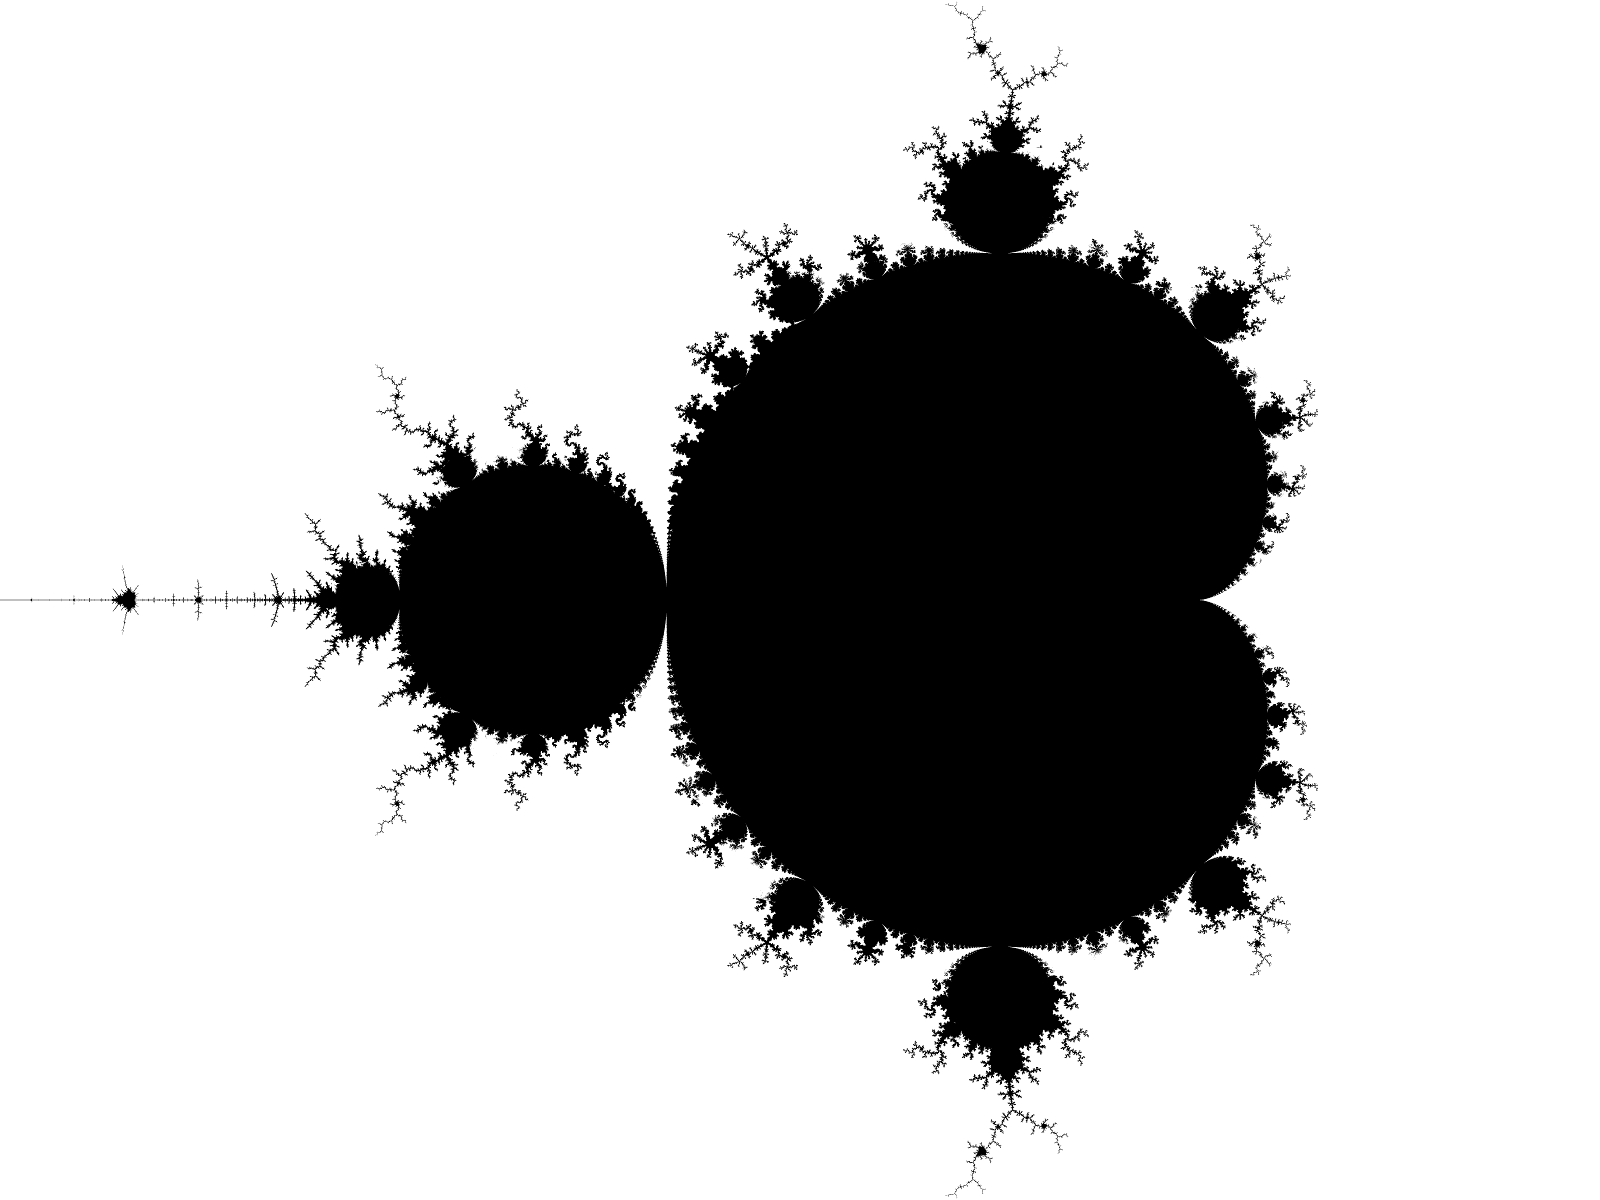
\includegraphics[width=\textwidth]{mandelbrot.png}
\end{center}
\caption{L'insieme di Mandelbrot generato al computer. Si veda il
codice a pagina \pageref{code:Mandelbrot}.}
\label{fig:mandelbrot}
\end{figure}

E' molto complicato determinare il carattere delle successioni definite
dal sistema~\eqref{eq:mandelbrot}.
Solo con l'utilizzo dei primi calcolatori
Mandelbrot (1924-2010) riuscì a rappresentare graficamente
\mymargin{insieme!di Mandelbrot}%
\index{Mandelbrot!insieme di}
l'insieme $M$ dei punti $c\in \CC$ per i quali la successione $z_n$ non diverge:
si veda la figura~\ref{fig:mandelbrot}.

Con l'esercizio~\ref{ex:mandelbrot_reale}
abbiamo trovato l'intersezione $M\cap \RR = [-2,1/4]$.
Nel seguente esercizio ci proponiamo ora di dimostrare un'altra semplice
proprietà che può essere
molto utile negli algoritmi numerici utilizzati per disegnare tale insieme.

\begin{exercise}[raggio di fuga]
Dimostrare che se $z_n$ è soluzione di \eqref{eq:mandelbrot}
se per un qualche $N\in \NN$ si ha $\abs{z_N}> 2$ allora $\abs{z_n}\to +\infty$
per $n\to +\infty$. In particolare l'insieme $M$ di Mandelbrot
è contenuto nel disco $\ENCLOSE{z\in \CC \colon \abs{z}\le 2}$.
\end{exercise}
%
\begin{proof}{Soluzione.}
Sia $c\in \CC$ fissato e si $z_n$ la successione definita da~\eqref{eq:mandelbrot}.
Per ogni $\eps>0$ consideriamo l'insieme:
\[
  A_\eps = \ENCLOSE{z \in \CC \colon \abs{z}\ge c \text{ e } \abs{z}\ge 2+\eps}.
\]
Possiamo mostrare che l'insieme $A_\eps$ è invariante in quanto se $z_n\in A_\eps$
si ha
\begin{equation}\label{eq:473244}
\begin{aligned}
\abs{z_{n+1}}
&= \abs{z_n^2+c}
\ge \abs{z_n}^2 - \abs{c}
\ge \abs{z_n}^2 - \abs{z_n}
= (\abs{z_n}-1)\abs{z_n}\\
&\ge (1+\eps)\abs{z_n}
\ge (1+\eps)(2+\eps)
\ge 2+\eps.
\end{aligned}
\end{equation}
Dunque $A_\eps$ è invariante ma non solo, se $z_n \in A_\eps$ abbiamo
trovato che risulta $\abs{z_{n+1}} \ge (1+\eps) \abs{z_n}$
e dunque $\abs{z_{n+k}} \ge (1+\eps)^k \abs{z_n}$ e dunque
$\abs{z_n}\to +\infty$ per $n\to +\infty$.

Se $\abs{c}\le 2$ e se $\abs{z_N}> 2$ allora $z_N \in A_\eps$ per
un qualche $\eps>0$ e dunque possiamo concludere che
$z_n\to \infty\in \bar \CC$.
Se invece $\abs{c}>2$ è facile osservare che $z_0 = 0$, $z_1=c$, $z_2=c^2+c$
e quindi
\[
  \abs{z_2}
    = \abs{c^2+c}
    \ge \abs{c}^2 - \abs{c}
    = \abs{c}(\abs{c}-1)
    \ge \abs{c} > 2
\]
dunque $z_2 \in A_\eps$ e quindi, comunque, $z_n\to \infty$.

\end{proof}
